\clearpage
\section{Wavelet Trees} \label{sec:wavelet_trees}
\todo[fancyline]{Improve this introduction, just a draft}
\noindent Wavelet trees, introduced in 2003 by Grossi, Gupta, and Vitter \cite{GrossiWT2003,} are a self indexing data structure: meaning they can answer rank and select queries, while still allowing to access the text. This combination makes them particularly useful for compressed full-text indexes like the FM-index \cite{ferragina2000opportunistic}. In such indexes, wavelet trees are employed to efficiently answer rank queries during the search process.

% Its name reflects its similarity to wavelet packet decomposition, where the sequence's "high" and "low" symbol values are separated and recursively subdivided.

\todo[inline, color=blue!30]{Upon closer examination, one can recognize that the wavelet tree is a slight extension of an older (1988) data structure by Chazelle \cite{Chazelle1988}, commonly used in Computational Geometry. This structure represents points on a two-dimensional grid, undergoing a reshuffling process to sort them by one coordinate and then by the other. Kärkkäinen (1999) \cite{karkkainen1999repetition} was the first to apply this structure to text indexing, although the concept and usage differed from Grossi et al.'s proposal four years later}

\noindent Wavelet Trees can be seen in different ways: (i) as sequence representation, (ii) as a permutation of elements, and (iii) as grid point representation. Since 2003, these perspectives and their interconnections have proven valuable across diverse problem domains, extending beyond text indexing and computational geometry, where the structure originated \cite{WTForALL,WTFromTheoryToPractice,TheMyriadVirtuesWT}.

\subsection*{An introduction to the problem}
Consider a sequence $S[1,n]$ as a generalization of bitvectors whose elements $S[i]$ are drawn from an alphabet $\Sigma$\footnote{The size of the alphabet varies depending on the application. For example, in DNA sequences, the alphabet is $\Sigma = \{A,C,G,T\}$ (in \autoref{ch:Chapter4} we will focus more on this specific case), while in other case it could be of millions of characters, such as in natural language processing.}. We are interested in the following operations on the sequence $S$:
\begin{itemize}
    \item \texttt{Access(i)}: return the $i$-th element of $S$.
    \item \texttt{Rank(c,i)}: return the number of occurrences of character $c$ in the prefix $S[1,i]$.
    \item \texttt{Select(c,i)}: return the position of the $i$-th occurrence of character $c$ in $S$.
\end{itemize}
However, dealing with sequences is much more complex than dealing with bitvectors (as we have seen in \autoref{sec:bitvectors}). In \cite{navarro2016compact} shows how a naive approach to solve this problem would require $n\sigma + o(n\sigma)$ bits of space, which is not space-efficient. Consider $\sigma$ bitvectors of length $n$, one for each symbol in the alphabet such that the $i$-th bit of the $c$-th bitvector is 1 if $S[i] = c$ and 0 otherwise. Then answering a $rank$ and $select$ query would be done by this simple transformation
\begin{align*}
    rank_c(S,i)   & = rank_1(B_c,i)   \\
    select_c(S,j) & = select_1(B_c,j)
\end{align*}
If we try to use the techniques from \autoref{sec:bitvectors} to compress the bitvectors, we would end up with a constant time complexity for the $rank$ and $select$ queries, but with the downside of a space occupancy of $n\sigma + o(n\sigma)$ bits. This is not space-efficient considering that the plain representation of the string requires $n\log \sigma + o(n)$ bits.\footnote{Even if we use a compressed representation of the bitvectors, the space occupancy would still have the dominant term $n\sigma$, that is at least $\Omega(n\sigma \log \log n / \log n)$ bits if we still want to support constant time $rank$ and $select$ queries.}
\begin{remark}[Notation]
    From now on, let $S[1,n]$ = $s_1s_2\dots s_n$ be a sequence of length $n$ over an alphabet $\Sigma$ that for simplicity we write as $\Sigma = \{1,\dots,\sigma\}$. In this way, the string can be represented using $n \lceil \log \sigma \rceil = n \log \sigma + o(n)$ bits in plain form.
\end{remark}

\subsection{Structure and construction}

In the beginning of this section we showed that storing one bitvector per symbol is not space-efficient. The wavelet tree is a data structure that solves this problem by using a recursive hierarchical partitioning of the alphabet. Consider the subset $[a,b] \subset [1, \dots, \sigma]$, then a wavelet tree over $[a,b]$ is a balanced binary tree with $b-a+1$ leaves\footnote{if $a=b$ then the tree is just a leaf}. The root node $v_{root}$ is associated with the whole sequence $S[1,n]$, and stores a bitmap $B_{v_{root}}[1,n]$ defined as follows: $B_{v_{root}}[i] = 0$ if $S[i] \leq (a+b)/2$ and $B_{v_{root}}[i] = 1$ otherwise. The tree is then recursively built by associating the subsequence $S_0[1,n_0]$ of elements in $[a, \dots,\lfloor (a+b)/2 \rfloor ]$ to the left child of $v$, and the subsequence $S_1[1,n_1]$ of elements in $[\lfloor (a+b)/2 \rfloor +1,\dots, b]$ to the right child of $v$. This process is repeated until the leaves are reached. In this way the left child of the root node, is a wavelet tree for $S_0[1,n_0]$ over the alphabet $[a,\dots, \lfloor (a+b)/2 \rfloor ]$, and the right child is a wavelet tree for $S_1[1,n_1]$ over the alphabet $[\lfloor (a+b)/2 \rfloor +1,\dots, b]$. \cite{WTForALL}

\noindent Building a wavelet tree is a recursive process that takes $O(n\log \sigma$) time by processing each node of the tree in linear time. The steps are outlined in Algorithm \ref{alg:build_wt}. Excluding the sequence $S$ and the final wavelet tree $T$, the algorithm uses $n \log \sigma$ bits of space \footnote{While building the wavelet tree, we can store the sequence $S$ on disk to free memory.}.

\clearpage
\begin{algorithm}[ht!]
    \caption{Building a wavelet tree}\label{alg:build_wt}
    \begin{algorithmic}
        % \Require Sequence $S[1,n]$ over alphabet $\Sigma = \{1,\dots,\sigma\}$
        % \Ensure Wavelet tree $T$ for $S$
        %

        \Function{build\_wt}{$S,n$}
        \State $T \gets build(S,n,1,\sigma)$
        \State \Return $T$
        \EndFunction


        \Function {build}{$S,n,a,b$} \Comment{\small{Takes a string $S[1,n]$ over $[a,b]$}}
        \If {$a = b$}
        \State Free S
        \State \Return null
        \EndIf
        \State $v \gets$ new node
        \State $m \gets \lfloor (a+b)/2 \rfloor$
        \State $z \gets 0$ \Comment{\small{number of elements in $S$ that are $\leq m$}}
        \For {$i \gets 1$ to $n$}
        \If {$S[i] \leq m$}
        \State $z \gets z+1$
        \EndIf
        \EndFor

        \State Allocate strings $S_{left}[1,z]$ and $S_{right}[1,n-z]$
        \State Allocate bitmap $v.B[1,n]$
        \State $z \gets 0$

        \For {$i \gets 1$ to $n$}
        \If {$S[i] \leq m$}
        \State \texttt{bitclear}($v.B,i$) \Comment{\small{set $i$-th bit of $v.B$ to 0}}
        \State $z \gets z+1$
        \State $S_{left}[z] \gets S[i]$
        \Else
        \State \texttt{bitset}($v.B,i$) \Comment{\small{set $i$-th bit of $v.B$ to 1}}
        \State $S_{right}[i-z] \gets S[i]$
        \EndIf
        \EndFor

        \State Free S
        \State $v.left \gets \texttt{build}(S_{left},z,a,m)$
        \State $v.right \gets \texttt{build}(S_{right},n-z,m+1,b)$
        \State Pre-process $v.B$ for $rank$ and $select$ queries
        \State \Return $v$
        \EndFunction
    \end{algorithmic}
\end{algorithm}

\begin{remark} \label{rem:space_occupancy_wavelet_tree}
    The wavelet tree described has $\sigma$ leaves and $\sigma-1$ internal nodes, and the height of the tree is $ \lceil \log \sigma \rceil$. The space occupancy of each level it's exactly $n$ bits, while we have at most $n$ bits for the last level. The total number of bits stored by the wavelet tree in then upper bounded by $n \lceil \log \sigma \rceil$ bits. \cite{WTForALL}. However, if we also interested in storing the topology of the wavelet tree, then another $O(\sigma \log n)$, that can be critical for large alphabets. In \cite{claude2011space,tischler2011wavelet} are presented some techniques to build wavelet tree in a space-efficient way.
\end{remark}

\begin{example}[Building a wavelet tree]
    Consider the sentence
    \begin{center}
        \texttt{wookies\_wield\_wicked\_weapons\_with\_wisdom\$}
    \end{center}
    where spaces are replaced by underscores and the sentence ends with a special character. The sorted alphabet for this example is
    \[
        \Sigma = \{\$, \_, a, c, d, e, h, i, k, l, m, n, o, p, s, t, w \}
    \]
    where we assume that in the lexicon the special character comes before the underscore. We now assign a bit to each symbol in the alphabet, where 0 is assigned to the first half of the alphabet and 1 to the second half.

    \begin{tabular}{*{17}{c}}
        \$                        & \_                        & a                         & c                         & d                         & e                         & h                         & i                         & k                         & l                         & m                         & n                         & o                         & p                         & s                         & t                         & w                         \\
        \textcolor{purple!100}{0} & \textcolor{purple!100}{0} & \textcolor{purple!100}{0} & \textcolor{purple!100}{0} & \textcolor{purple!100}{0} & \textcolor{purple!100}{0} & \textcolor{purple!100}{0} & \textcolor{purple!100}{0} & \textcolor{purple!100}{1} & \textcolor{purple!100}{1} & \textcolor{purple!100}{1} & \textcolor{purple!100}{1} & \textcolor{purple!100}{1} & \textcolor{purple!100}{1} & \textcolor{purple!100}{1} & \textcolor{purple!100}{1} & \textcolor{purple!100}{1} \\
    \end{tabular}

    \noindent We can now build the wavelet tree for this sequence, recursively partitioning the alphabet and assigning a bit to each symbol. The resulting wavelet tree is shown in \autoref{fig:wavelet_tree_example}

\end{example}

\begin{figure}[h]
    \centering
    \tikzstyle{every node}=[font=\footnotesize]
    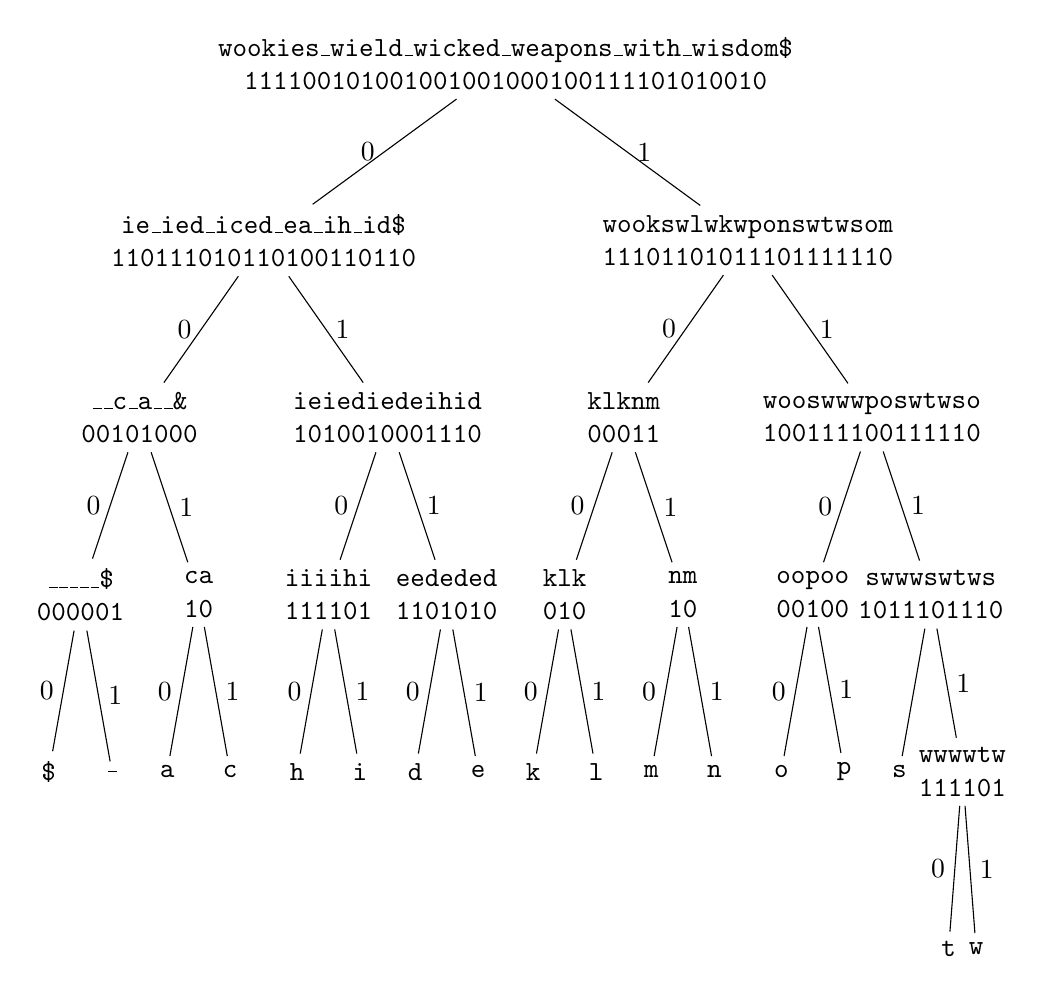
\begin{tikzpicture}[
            scale=0.5,
            level distance=4.5cm,
            level 1/.style={sibling distance=12.3cm},
            level 2/.style={sibling distance=6.3cm},
            level 3/.style={sibling distance=3cm},
            level 4/.style={sibling distance=1.6cm},
            level 5/.style={sibling distance=0.7cm},
            level 6/.style={sibling distance=0.7cm},
            level 7/.style={sibling distance=0.7cm}]  % Added level 7 style
        \node[align=center] {\texttt{wookies\_wield\_wicked\_weapons\_with\_wisdom\$}\\\texttt{111100101001001001000100111101010010}}
        child {node[align=center] {\texttt{ie\_ied\_iced\_ea\_ih\_id\$}\\\texttt{110111010110100110110}}
                child {node[align=center] {\texttt{\_\_c\_a\_\_\&}\\\texttt{00101000}}
                        child {node[align=center] {\texttt{\_\_\_\_\_\$}\\\texttt{000001}}
                                child {node[align=center] {\texttt{\$}} edge from parent node[left] {0}}  % Added level 7 node
                                child {node[align=center] {\texttt{\_}} edge from parent node[right] {1}}  % Added level 7 node
                                edge from parent node[left] {0}}
                        child {node[align=center] {\texttt{ca}\\\texttt{10}}
                                child {node[align=center] {\texttt{a}} edge from parent node[left] {0}}  % Added level 7 node
                                child {node[align=center] {\texttt{c}} edge from parent node[right] {1}}  % Added level 7 node
                                edge from parent node[right] {1}}
                        edge from parent node[left] {0}}
                child {node[align=center] {\texttt{ieiediedeihid}\\\texttt{1010010001110}}
                        child {node[align=center] {\texttt{iiiihi}\\\texttt{111101}}
                                child {node[align=center] {\texttt{h}} edge from parent node[left] {0}}  % Added level 7 node
                                child {node[align=center] {\texttt{i}} edge from parent node[right] {1}}  % Added level 7 node
                                edge from parent node[left] {0}}
                        child {node[align=center] {\texttt{eededed}\\\texttt{1101010}}
                                child {node[align=center] {\texttt{d}} edge from parent node[left] {0}}  % Added level 7 node
                                child {node[align=center] {\texttt{e}} edge from parent node[right] {1}}  % Added level 7 node
                                edge from parent node[right] {1}}
                        edge from parent node[right] {1}}
                edge from parent node[left] {0}}
        child {node[align=center] {\texttt{wookswlwkwponswtwsom}\\\texttt{11101101011101111110}}
                child {node[align=center] {\texttt{klknm}\\\texttt{00011}}
                        child {node[align=center] {\texttt{klk}\\\texttt{010}}
                                child {node[align=center] {\texttt{k}} edge from parent node[left] {0}}  % Added level 7 node
                                child {node[align=center] {\texttt{l}} edge from parent node[right] {1}}  % Added level 7 node
                                edge from parent node[left] {0}}
                        child {node[align=center] {\texttt{nm}\\\texttt{10}}
                                child {node[align=center] {\texttt{m}} edge from parent node[left] {0}}  % Added level 7 node
                                child {node[align=center] {\texttt{n}} edge from parent node[right] {1}}  % Added level 7 node
                                edge from parent node[right] {1}}
                        edge from parent node[left] {0}}
                child {node[align=center] {\texttt{wooswwwposwtwso}\\\texttt{100111100111110}}
                        child {node[align=center] {\texttt{oopoo}\\\texttt{00100}}
                                child {node[align=center] {\texttt{o}} edge from parent node[left] {0}}  % Added level 7 node
                                child {node[align=center] {\texttt{p}} edge from parent node[right] {1}}  % Added level 7 node
                                edge from parent node[left] {0}}
                        child {node[align=center] {\texttt{swwwswtws}\\\texttt{1011101110}}
                                child {node[align=center] {\texttt{s}}}
                                child {node[align=center] {\texttt{wwwwtw}\\\texttt{111101}}
                                        child {node[align=center] {\texttt{t}} edge from parent node[left] {0}}  % Added level 7 node
                                        child {node[align=center] {\texttt{w}} edge from parent node[right] {1}}  % Added level 7 node
                                        edge from parent node[right] {1}}
                                edge from parent node[right] {1}}
                        edge from parent node[right] {1}}
                edge from parent node[right] {1}};
    \end{tikzpicture}
    \caption{\small Wavelet tree for the sequence \texttt{wookies\_wield\_\dots}} \label{fig:wavelet_tree_example}
\end{figure}

\subsubsection*{Tracking symbols}
We have seen how the wavelet tree serves as a representation for a string $S$, but more than that it is a succinct data structure for the string. Thus, it takes space asymptotically close to the plain representation of the string and allows us to access the $i$-th symbol of the string in $O(\log \sigma)$ time.

\subsubsection{Access}
In algorithm \ref{alg:access_wt} we show how extract the $i$-th symbol of the string $S$ using a wavelet tree $T$, this operation is called \texttt{Access}. In order to find $S[i]$, we first look at the bitmap associated with the root node of the wavelet tree, and depending on the value of the $i$-th bit of the bitmap, we move to the left or right child of the root node and continue recursively. However, the problem is to determine where our $i$ has been mapped to: if we move to the left child, then we need to find the $i$-th 0 in the bitmap of the left child, and if we move to the right child, then we need to find the $i$-th 1 in the bitmap of the right child. This is done by the $rank_0$ and $rank_1$ functions, respectively. We continue this process until we reach a leaf node, and then we return the value of the leaf node.

\begin{algorithm}[h!]
    \caption{\texttt{Access} queries on a wavelet tree}\label{alg:access_wt}
    \begin{algorithmic}
        \Function {access}{$T,i$} \Comment{\small{$T$ is the sequence $S$ seen as a wavelet tree}}
        \State $v \gets T_{root}$ \Comment{\small{start at the root node}}
        \State $[a,b] \gets [1,\sigma]$
        \While{$a \neq b$}
        \If{$access(v.B,i) =0$} \Comment{\small{$i$-th bit of the bitmap of $v$}}
        \State $i \gets rank_0(v.B,i)$
        \State $v \gets v.left$ \Comment{\small{move to the left child of node $v$}}
        \State $b \gets \lfloor (a+b)/2 \rfloor$
        \Else
        \State $i \gets rank_1(v.B,i)$
        \State $v \gets v.right$ \Comment{\small{move to the right child of node $v$}}
        \State $a \gets \lfloor (a+b)/2 \rfloor +1$
        \EndIf
        \EndWhile
        \State \Return $a$
        \EndFunction
    \end{algorithmic}
\end{algorithm}


\subsubsection{Select}
In addition to retrieving the $i$-th symbol of the string, we might also need to perform the inverse operation. That is, given a symbol's position at a leaf node, we aim to determine the position of the symbol in the string. This operation is referred to as \texttt{Select} and is outlined in Algorithm \ref{alg:select_wt}. Assume we start at a given leaf node $v$ and want to find the position of the $j$-th occurrence of symbol $c$ in the string. We recursively move to the left or right child of the node $v$: if the leaf is the right child of its parent, then we need to find the $j$-th 1 in the bitmap of the parent node, and if the leaf is the left child of its parent, then we need to find the $j$-th 0 in the bitmap of the parent node. This is done by the $select_0$ and $select_1$ functions, respectively. We continue this process until we reach the root node, and then we return the position of the symbol in the string. As we have seen in \autoref{sec:bitvectors}, this two single operations can be solved in constant time if we use the \texttt{RRR} data structure \cite{RRR2002} on each bitmap. Thus, the time complexity to perform a \texttt{Select} query on a wavelet tree is $O(\log \sigma)$.

\begin{algorithm}
    \caption{\texttt{Select} queries on a wavelet tree}\label{alg:select_wt}
    \begin{algorithmic}
        % add two functions to the algorithmic environment
        \Function{$\text{select}_c$}{$S,j$}
        % \Require Sequence $S$ (as a wavelet tree $T$), symbol $c$, position $j$
        % \Ensure The position of the $j$-th occurrence of $c$ in $S$

        \State \Return $\text{select}(T._{root},1, \sigma, c, j)$
        \EndFunction



        \Function{$\text{select}$}{$v,a,b,c,j$}
        % \Comment $v$ is the current node, $[a,b]$ is the alphabet range, $c$ is the symbol, $j$ is the position
        \If{$a = b$}
        \State \Return $j$
        \EndIf

        \If {$c \leq \lfloor (a+b)/2 \rfloor$}
        \State $j$ $\gets$ $\text{select}(v.left, a, \lfloor (a+b)/2 \rfloor, c, j)$
        \Return $select_0(v.B,j)$

        \Else
        \State $j$ $\gets$ $\text{select}(v.right, \lfloor (a+b)/2 \rfloor +1, b, c, j)$
        \State \Return $select_1(v.B,j)$
        \EndIf

        \EndFunction

    \end{algorithmic}
\end{algorithm}

\subsubsection{Rank} During the $select$ algorithm, we track upwards the path from the leaf to the root. The process for solving a $rank$ query is similar, but instead of moving from the leaf to the root, we move from the root to the leaf. Algorithm \ref{alg:access_wt} also gives us the number of occurrences of a symbol $S[i]$ in the prefix $S[1,i]$, i.e $rank_{S[i]}(S,i)$. We now want to generalize this operation to solve any rank query $rank_c(S,i)$, where $c$ is a symbol in the alphabet. This procedure is shown in \ref{alg:rank_wt}.
\begin{algorithm}[h!]
    \caption{\texttt{Rank} queries on a wavelet tree}\label{alg:rank_wt}
    \begin{algorithmic}
        \Function{$\text{rank}_c$}{$S,i$}
        \State $v \gets T_{root}$ \Comment{\small{start at the root node}}
        \State $[a,b] \gets [1,\sigma]$
        \While {$a \neq b$}
        \If {$c \leq \lfloor (a+b)/2 \rfloor$}
        \State $i \gets rank_0(v.B,i)$
        \State $v \gets v.left$ \Comment{\small{move to the left child of node $v$}}
        \State $b \gets \lfloor (a+b)/2 \rfloor$
        \Else
        \State $i \gets rank_1(v.B,i)$
        \State $v \gets v.right$ \Comment{\small{move to the right child of node $v$}}
        \State $a \gets \lfloor (a+b)/2 \rfloor +1$
        \EndIf
        \EndWhile
        \State \Return $i$
        \EndFunction
    \end{algorithmic}

\end{algorithm}

% \noindent TODO: Add some pratical consideration about using constant-time $rank$ and $select$ on the bitvectors. \cite{navarro2016compact} 6.2

\todo[inline, color=blue!30]{
    TBD if to add: In \ref{rem:space_occupancy_wavelet_tree} we mentioned that storing the topology of the wavelet tree requires $O(\sigma \log n)$ bits. This may be critical for large alphabets, and in this section we will show that this term can be removed by slightly altering the balanced wavelet tree shape. \cite{MAKINEN2007332,MAKINEN2006703}.

    Look for section 2.3 of \cite{WTForALL}
}

\clearpage
\subsection{Compressed Wavelet Trees} \label{sec:compressed_WT}
In order to make the wavelet tree more space efficient, we ask ourselves if we can compress this data structure. The answer is yes, and in this section we will see how a wavelet tree can be compressed to the zero-order entropy of the input string, while still being able to answer rank and select queries in $O(\log \sigma)$ time. The literature on this topic mainly focus one two different approaches: compressing the bitvectors and altering the shape of the wavelet tree itself.

\subsubsection{Compressing the bitvectors} \label{subsec:compressing_bitvectors}
In \cite{GrossiWT2003} Grossi et. al showed that if the bitvectors of each single node are compressed to their zero-order entropy, then their overall space occupance is $n H_0(S)$. So if we suppose that the bitmap associated to the root node has a skewed distribution of $0$s and $1$s, then the zero-order compressing it yields a space of
\begin{equation}
    n_0 \log \frac{n}{n_0} + n_1 \log \frac{n}{n_1}
\end{equation}
where $n_0$ and $n_1$ are the number of $0$s and $1$s in the bitmap, respectively. This is the same as the zero-order entropy of the bitmap. The same reasoning can be applied to the bitmaps of the children of the root node, and so on. This way, one can easy prove by induction \cite{navarro2016compact} that the overall space of the wavelet tree is
\begin{equation}
    \sum_{c \in \Sigma} n_c \log (\frac{n}{n_c}) = n H_0(S)
\end{equation}
% However, to this quantity we must add the redundancy, i.e the space occupied by the pointers of the tree. This redundancy is $o(n \log \sigma)$. Thus bringing the space occupance of the wavelet tree to $n H_0(S) + o(n \log \sigma)$.\todo{I'm not sure that this is true, navarro says that there should be also a $+ O(\sigma w)$ term, but I don't know where it comes from.}

\noindent We can now choose from the literature any zero-order entropy coding method for the bitvectors that supports rank and select queries in $O(1)$ time. Some of the most popular methods are RRR \cite{RRR2002} that we have vastly discussed in \autoref{sec:bitvectors}, that for each bitvector of length $n$ uses $n H_0(B) + o(n \log \log n / \log n)$ bits. In \cite{patrascu2008succincter} the authors showed\footnote{In this case, the time complexity of rank and select queries is $O(c)$.} that this value can be further reduced to $n H_0(B) + o(n/\log^c n)$ for any positive constant $c$.

\subsubsection{Huffman-Shaped Wavelet Trees}
Since working in practice with compressed bitvectors can be less efficient then in theory, we want a method for still obtaining nearly zero-order entropy compression, but while maintaining the bitvectors in plain form. The key idea for the compression method that we are going to analyze is that, as noted by Grossi et. al in \cite{grossi2004indexing}, the shape of the wavelet tree has no impact on the space occupance of the structure. They proposed to use this fact to alter the shape of the tree in order to optimize the average query time. Recalling how we built an Huffman Tree in \ref{subsec:huffman_coding}, we can adapt the same idea to the wavelet tree: given the frequencies $f_c$ with which each leaf node appears in the tree, we can create an Huffman-shaped wavelet tree, obtaining an average access time of
\begin{equation}
    \sum_{c \in \Sigma} f_c \log \frac{1}{f_c} \leq \log \sigma
\end{equation}
A counter effect noted by the authors in \cite{grossi2004indexing} is that in the worst case, we could and up with a time complexity of $O(\log n)$, for example in the case of a very infrequent symbol.However, if we choose $i$ uniformly at random from $[1, n]$ then the average access\footnote{And also for $rank_c(S,j)$ or $select_c(S,j)$ with $c = S=[1]$} time is
\begin{equation}
    O(\frac{1}{n} \sum_c f_c |h(c)| = O(1 + H_0(S))
\end{equation}
That is better than the $O(\log \sigma)$ time of the original balanced wavelet tree.

\begin{remark}
    On a further note, if we bound the depth of the Huffman Tree, we can keep worst care access time to $O(\log \sigma)$, with extra $O(n/\sigma)$ bits of redundancy
\end{remark}

\noindent Another possibile approach following the same idea of a Huffman-shaped wavelet tree, proposed in \cite{makinen2004new}, is to use the frequencies with which the symbols appear in the string. If we use this frequencies to build the Huffman Tree, we can then attach to each node $v$ a bitvector $B_v$ in the same way that we would do for the balanced wavelet tree (\ref{alg:build_wt}). In this way, the bits of $B_v$ are the bits of of the path from the root to $v$ in the Huffman Tree, i.e the Huffman codes of the symbols. Let's see the space occupance of this structure. Consider a leaf corresponding to a symbol $c$, at depth $|h(c|)$ (where $h(c)$ is the bitwise Huffman code for $c$), representing $f_c$ symbols. Each of this occurrences leads to a bit in each bitvector that is in the path from the root to the leaf; that is $|h(c)|$ bits. Thus, the occurrences of $c$ lead to $f_c |h(c)|$ bits in total. If we add this values to all the leaves we obtain same number of bits outputted by the Huffman coding of the string, that is
\begin{equation}
    \sum_{c \in \Sigma} f_c |h(c)| \leq n(H_0(S) + 1)
\end{equation}
If we also want to add the space to support the rank and select queries and the tree pointers needed to navigate the tree, we arrive to a space occupance of
\begin{equation}
    n(H_0(S) + 1) + o(n(H_0(S) + 1)) + O(n \log \sigma)
\end{equation}
For the sake of completeness, we also mention that the shape of an Huffman tree is not the only one that can be given to a wavelet tree. In \cite{grossi2012wavelet} Grossi and Ottaviano gave the wavelet the shape of a trie, making it possible to handle a sequence of strings.

\subsubsection{Higher Order Entropy Coding}

\todo[inline, color=blue!20]{TODO and TBD: Ask Grossi how in depth to go with this section, Ferragina and Manzini in \cite{TheMyriadVirtuesWT} give a very technical explanation of the method. While in \cite{WTForALL} Navarro gives a more high-level explanation. Furthermore, all this methods relies on the BTW transform, which is not covered in this thesis, do I add a section on it?}
